% This is a Basic Assignment Paper but with like Code and stuff allowed in it, there is also url, hyperlinks from contents included. 

\documentclass[11pt]{article}

% Preamble

\usepackage[margin=1in]{geometry}
\usepackage{amsfonts, amsmath, amssymb}
\usepackage{fancyhdr, float, graphicx}
\usepackage[utf8]{inputenc} % Required for inputting international characters
\usepackage[T1]{fontenc} % Output font encoding for international characters
\usepackage{fouriernc} % Use the New Century Schoolbook font
\usepackage[nottoc, notlot, notlof]{tocbibind}
\usepackage{listings}
\usepackage{xcolor}
\usepackage{blindtext}
\usepackage{hyperref}
\hypersetup{
    colorlinks=true,
    linkcolor=black,
    filecolor=magenta,      
    urlcolor=cyan,
    pdfpagemode=FullScreen,
    }

\definecolor{codegreen}{rgb}{0,0.6,0}
\definecolor{codegray}{rgb}{0.5,0.5,0.5}
\definecolor{codepurple}{rgb}{0.58,0,0.82}
\definecolor{backcolour}{rgb}{0.95,0.95,0.92}

\lstdefinestyle{mystyle}{
    backgroundcolor=\color{backcolour},   
    commentstyle=\color{codegreen},
    keywordstyle=\color{magenta},
    numberstyle=\tiny\color{codegray},
    stringstyle=\color{codepurple},
    basicstyle=\ttfamily\footnotesize,
    breakatwhitespace=false,         
    breaklines=true,                 
    captionpos=b,                    
    keepspaces=true,                 
    numbers=left,                    
    numbersep=5pt,                  
    showspaces=false,                
    showstringspaces=false,
    showtabs=false,                  
    tabsize=2
}

\lstset{style=mystyle}

% Header and Footer
\pagestyle{fancy}
\fancyhead{}
\fancyfoot{}
\fancyhead[L]{\textit{\Large{SET Assignment 6 - Activity and State diagrams}}}
%\fancyhead[R]{\textit{something}}
\fancyfoot[C]{\thepage}
\renewcommand{\footrulewidth}{1pt}



% Other Doc Editing
% \parindent 0ex
%\renewcommand{\baselinestretch}{1.5}

\begin{document}

\begin{titlepage}
	\centering

	%---------------------------NAMES-------------------------------

	\huge\textsc{
		MIT World Peace University
	}\\

	\vspace{0.75\baselineskip} % space after Uni Name

	\LARGE{
		Software Engineering and Testing\\
		Second Year B. Tech, Semester 4
	}

	\vfill % space after Sub Name

	%--------------------------TITLE-------------------------------

	\rule{\textwidth}{1.6pt}\vspace*{-\baselineskip}\vspace*{2pt}
	\rule{\textwidth}{0.6pt}
	\vspace{0.75\baselineskip} % Whitespace above the title



	\huge{\textsc{
			Activity and State Diagrams
		}} \\



	\vspace{0.5\baselineskip} % Whitespace below the title
	\rule{\textwidth}{0.6pt}\vspace*{-\baselineskip}\vspace*{2.8pt}
	\rule{\textwidth}{1.6pt}

	\vspace{1\baselineskip} % Whitespace after the title block

	%--------------------------SUBTITLE --------------------------	

	\LARGE\textsc{
		\centering
		Assignment 6
	} % Subtitle or further description
	\vfill

	%--------------------------AUTHOR-------------------------------

	Prepared By
	\vspace{0.5\baselineskip} % Whitespace before the editors

	\Large{
		Krishnaraj Thadesar \\
		Cyber Security and Forensics\\
		Batch A1, PA 20
	}


	\vspace{0.5\baselineskip} % Whitespace below the editor list
	\today

\end{titlepage}


\tableofcontents
\thispagestyle{empty}
\clearpage

\setcounter{page}{1}

\section{Aim}
Object Oriented Analysis and design using UML diagrams: Activity and State Chart
diagram, using Open Source Tool.

\section{Objectives}
\begin{enumerate}
	\item To learn the relationships and notions of Activity diagram.
	\item To learn the relationships and notions of State Chart diagram.
\end{enumerate}

\section{Problem Statement}

\textbf{Draw Activtiy Diagram and State Diagram for The Following Problem:} \\

\textit{The Purpose of an Attandence Assistant App is to help reduce the time taken for recording the attendance of a classroom in a school or college. The app will be able to record the attendance of a class in a matter of a few Seconds with minimum Energy Expended. It will record data on cloud, and be accessible to all the Teachers.}\\

The tasks we have to do are:
\begin{enumerate}
	\item You will have to identify the main entities (objects) for this system.
	\item You will have to find out the relationships between these objects.
	\item You will have to find the necessary attributes and functions that need to be associated
	      with each object to implement the functionality mentioned above.
	\item You will make a final comprehensive diagram show and all objects and their relations
	      along with their attributes and functions.
\end{enumerate}

\section{Theory}
% describe and explain the notions and stuff used to draw the activity and state diagram, also attack their images. 

\subsection{State Diagram}

\subsubsection{What is a State Diagram}

\textit{A state diagram is a type of behavioral diagram that shows the flow of control from one state to another. A state diagram is a dynamic diagram because it shows the behavior of the system.}

\subsubsection{What is the use of a State Diagram}

\begin{enumerate}
	\item \textit{Describing the behavior of a system}: A state diagram can be used to describe the behavior of a system, including the various states the system can be in and the transitions between those states.

	\item \textit{Modeling complex systems}: A state diagram can be used to model complex systems and help identify potential problems or errors in the system's design.

	\item \textit{Designing software programs}: State diagrams can be used in software design to map out the different states of a program and the actions that occur during transitions between those states.

	\item \textit{Understanding complex processes}: State diagrams can be used to help understand complex processes, such as manufacturing or logistics processes, by breaking them down into smaller, more manageable steps.

	\item \textit{Communicating ideas}: State diagrams are a useful tool for communicating ideas and concepts to others, as they provide a visual representation of a process or system that can be easily understood.
\end{enumerate}


\subsubsection{Elements of a State Diagram}

\begin{enumerate}
	\item \textbf{State:} A state is a situation in which a system is in a particular condition. It is a scenario that describes the interaction between a user and a system to achieve a particular goal. A state is represented as a rectangle in a state diagram.
	\item \textbf{Flow of Control:} Flow of control is the direction of the flow of control from one state to another. It is represented as a line with an arrowhead. The arrowhead points in the direction of the flow of control.
	\item \textbf{Initial State:} The initial state is the state in which a system is present at the beginning of a scenario. It is represented as a circle in a state diagram.
	\item \textbf{Final State:} The final state is the state in which a system is present at the end of a scenario. It is represented as a double circle in a state diagram.
	\item \textbf{Transition:} A transition is a change from one state to another. It is represented as a line with an arrowhead. The arrowhead points in the direction of the flow of control.
\end{enumerate}

\begin{figure}[H]
	\centering
	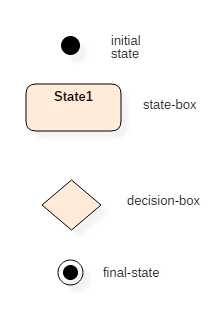
\includegraphics[width=0.35\textwidth]{052919_0832_StateMachin1.png}
	\caption{State Diagram Elements}
	\label{fig:state_diagram}
\end{figure}

\subsubsection{State Diagram for the Problem Statement}

\begin{figure}[H]
	\centering
	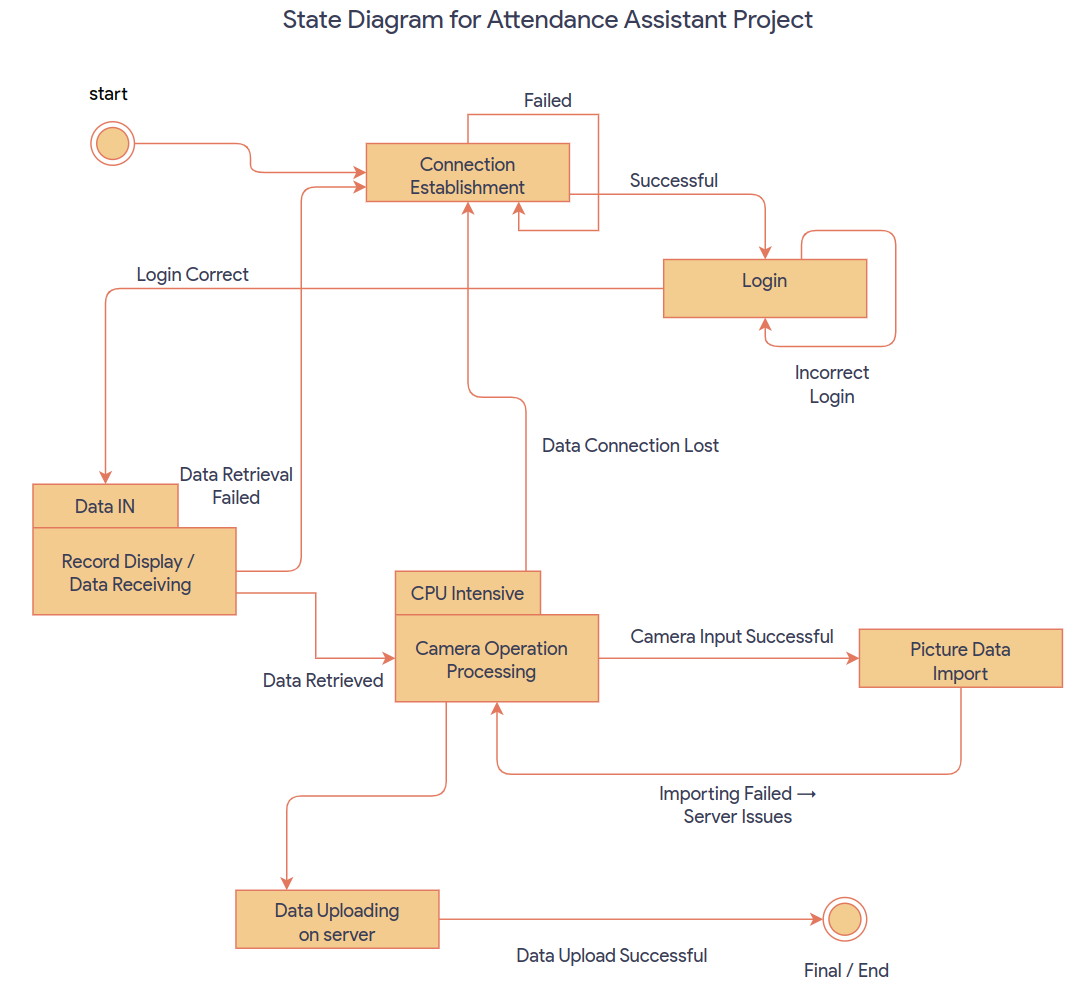
\includegraphics[width=0.95\textwidth]{state.png}
	\caption{State Diagram for the Problem Statement}
	\label{fig:state_diagram_problem_statement}
\end{figure}

\clearpage

\subsection{Activity Diagram}

\subsubsection{What is an Activity Diagram}

\textit{An activity diagram is a type of behavioral diagram that shows the flow of control from one activity to another. An activity diagram is a dynamic diagram because it shows the behavior of the system.}

\subsubsection{What is the use of an Activity Diagram}

\begin{enumerate}
	\item \textit{Modeling business processes}: Activity diagrams can be used to model business processes, helping to visualize and analyze the flow of information and tasks between different departments and stakeholders.
	\item \textit{Software design}: Activity diagrams are used to model the behavior of software systems, such as software modules or classes, and to visualize how the system will interact with users or other systems.
	\item \textit{Analyzing workflows}: Activity diagrams can be used to analyze workflows within an organization, identifying inefficiencies and areas for improvement.
	\item \textit{Communication}: Activity diagrams are a powerful tool for communicating ideas and processes to stakeholders and team members, providing a visual representation of complex processes that is easy to understand.
	\item \textit{Testing and quality assurance}: Activity diagrams can be used in testing and quality assurance to ensure that software systems and business processes are working as intended and to identify potential problems or bottlenecks.
\end{enumerate}

\subsubsection{Elements of an Activity Diagram}

\begin{enumerate}
	\item \textbf{Activity:} An activity is a set of actions that are performed to achieve a goal. It is a scenario that describes the interaction between a user and a system to achieve a particular goal. An activity is represented as a rectangle in an activity diagram.
	\item \textbf{Flow of Control:} Flow of control is the direction of the flow of control from one activity to another. It is represented as a line with an arrowhead. The arrowhead points in the direction of the flow of control.
	\item \textbf{Decision:} Decision is a decision point in the activity diagram. It is represented as a diamond in an activity diagram.
	\item \textbf{Fork:} Fork is a point in the activity diagram where the flow of control splits into two or more parallel paths. It is represented as a circle with a line through it in an activity diagram.
	\item \textbf{Join:} Join is a point in the activity diagram where the flow of control joins from two or more parallel paths. It is represented as a circle with a line through it in an activity diagram.
	\item \textbf{Initial Node:} Initial node is the starting point of the activity diagram. It is represented as a circle in an activity diagram.
	\item \textbf{Final Node:} Final node is the ending point of the activity diagram. It is represented as a circle in an activity diagram.
\end{enumerate}

\begin{figure}[H]
	\centering
	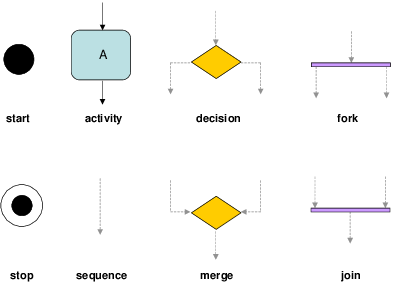
\includegraphics[width=.8\textwidth]{UML-Activity-Diagram-elements.png}
	\caption{Activity Diagram Elements}
\end{figure}

\clearpage
\subsection{Diagram for the Problem Statement}

\begin{figure}[H]
	\centering
	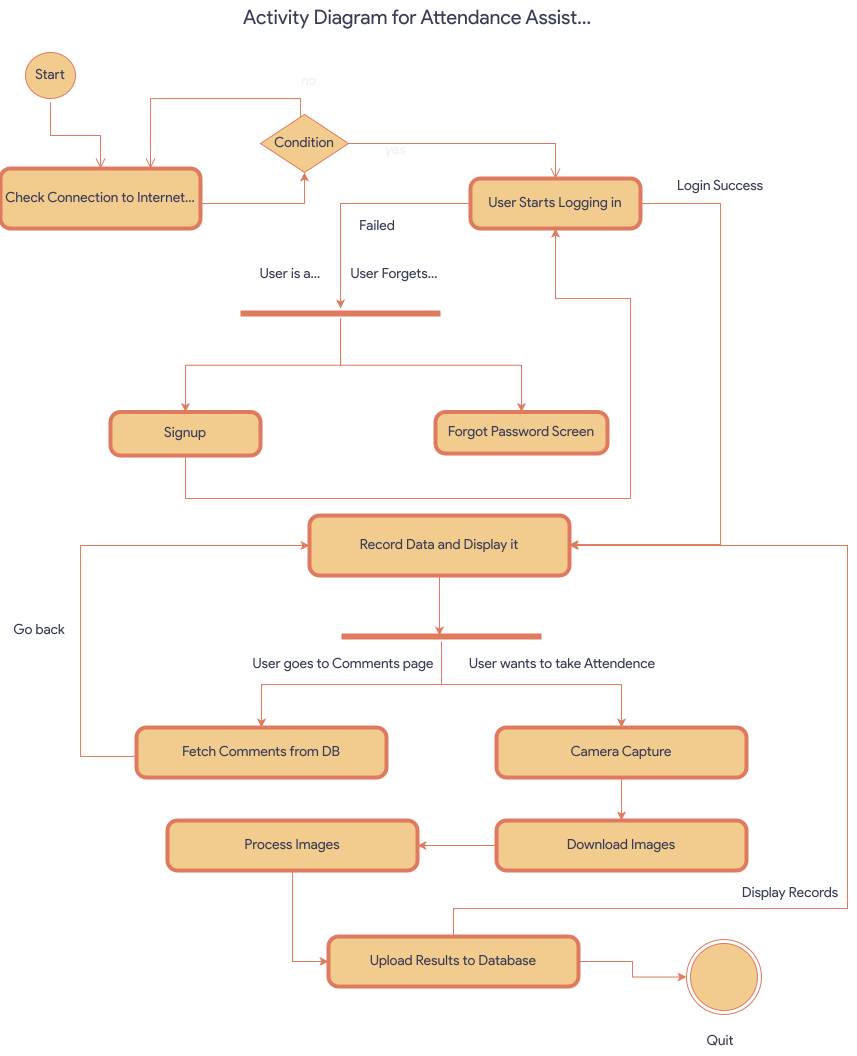
\includegraphics[width=0.95\textwidth]{activity dia.drawio.png}
	\caption{Activity Diagram for the Problem Statement}
\end{figure}
\section{Platform}
\textbf{Operating System}: Arch Linux x86-64 \\
\textbf{IDEs or Text Editors Used}: Visual Studio Code\\
\textbf{External Programs for Diagrams} : Draw.io\\


\section{Conclusion}
Thus, we learnt about Use case diagrams, and UML Class diagrams in detail.
\clearpage

\section{FAQ}
\begin{enumerate}
	\item \textbf{Give the significance of Activity diagram.}\\

	      Activity diagrams are an important modeling tool in software development as they allow developers to visually represent the flow of activities and actions within a system. Some of the key significances of activity diagrams are:

	      \begin{enumerate}
		      \item They help to identify the sequence of activities and actions that are involved in a process, making it easier to understand and optimize the process.
		      \item They help to identify the different actors or roles involved in a process, and how they interact with each other.
		      \item They help to identify the various conditions and decision points that exist in a process, and how they affect the flow of activities.
		      \item They can be used to communicate complex processes and workflows to stakeholders, making it easier for them to understand and provide feedback.
	      \end{enumerate}

	\item \textbf{Explain any 2 terminologies used in Activity diagrams.}\\

	      \begin{enumerate}
		      \item Action: An action is a single step or operation that is performed as part of an activity. It represents a specific behavior that is performed by an object, system, or actor. Actions are represented by rectangular shapes with rounded corners in an activity diagram.
		      \item Decision node: A decision node is used to represent a decision point in an activity diagram. It is represented by a diamond-shaped symbol with multiple outgoing edges. The edges represent the different possible paths that can be taken based on the outcome of the decision.
	      \end{enumerate}

	\item \textbf{Explain the message passing in State Chart diagram.}\\
	Message passing is a key concept in state chart diagrams. It is used to model the communication and interaction between different objects or entities in a system. In a state chart diagram, message passing is represented using arrows between states, with the arrows labeled with the message that is being passed.\\

	When an object or entity sends a message to another object or entity, it can trigger a transition from one state to another. The receiving object or entity can then process the message and respond accordingly, which can cause further state transitions.
	
	
	\item \textbf{Illustrate the use of a state diagram, consider software embedded within the Safe Home control panel that is responsible for reading user input}\\

\end{enumerate}

\end{document}